\documentclass[12pt,letterpaper]{article}
\usepackage{amsmath}
\usepackage{amsfonts}
\usepackage{amssymb}
\usepackage{enumitem}
\usepackage[left=2cm,right=2cm,top=3cm,bottom=3cm]{geometry}
\usepackage{natbib}
\usepackage{graphicx}
\usepackage{xcolor}
\usepackage[colorlinks = true,
            linkcolor = blue,
            urlcolor  = blue,
            citecolor = blue,
            anchorcolor = blue]{hyperref}

\newcommand{\MYhref}[3][blue]{\href{#2}{\color{#1}{#3}}}%

\def\wl{\par \vspace{\baselineskip}}

\author{Abel Flores Prieto}
\title{Capstone Project Write Up - Cosmic Microwave Background Data}

\begin{document}
\maketitle

\section*{Scope}
This project focuses on the data used for computing the Cosmic Microwave
Background or CMB (see Figure \ref{fig:cmb}). In this project I focus to easily
enable access to data used for computing the CMB. The data used for this
project is simulated by \MYhref{https://arxiv.org/abs/0908.0540}{Sehgal et al.
(2010)} and can be found
\MYhref{https://lambda.gsfc.nasa.gov/simulation/tb\_sim\_ov.cfm}{here}. This
simulated data works as a tool to cross-check multiple calculations from real
surveys, including power spectrum calculations.

\begin{figure}[h!]
    \centering
    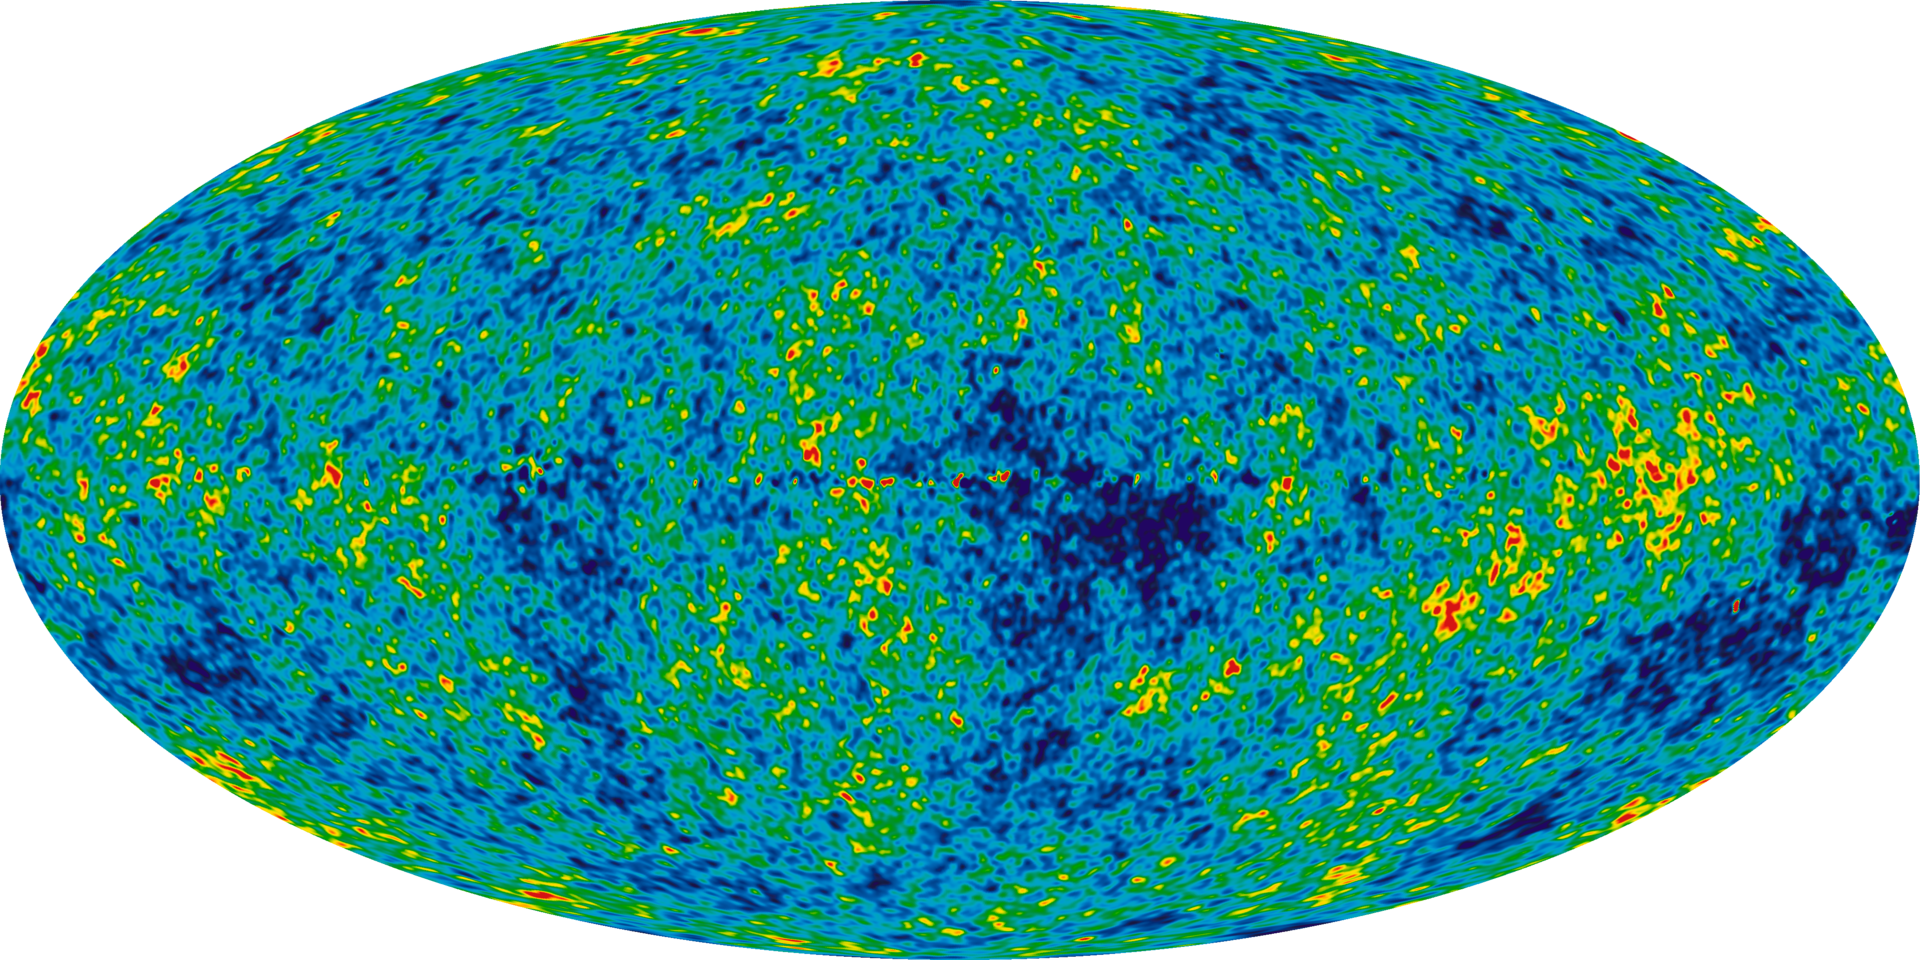
\includegraphics[width=0.75\textwidth]{imgs/cmb_temp.png}
    \caption{Cosmic Microwave Background temperature, remnant of the beginning
    of the universe. Image generated by NASA.}
    \label{fig:cmb}
\end{figure}

The data can be downloaded from the \MYhref{https://lambda.gsfc.nasa.gov}{Legacy
Archive for Microwave Background Data Analysis}. The data used in this project
is simulated by a team of researchers and includes realistic simulations of the
microwave sky. The data is composed of Halo Catalogs and Galaxy Catalogs.

The end solution of the project is to have a data lake in S3 so that I, or
anyone (with the right permissions) can access the data for further processing.
The data lake will sit in one of my S3 buckets,
\texttt{s3://abelfp-physics-data/} and will have two main tables, with the
possibility to expand: \texttt{cmb\_simulated} for simulated galaxy catalogs,
and \texttt{halo\_simulated} for the halo catalogs.
The galaxy catalogs come in DAT files with over 80 GB of data while the halo
catalogs come in as ASCII.GZ files with over 800 MB of data. All of this data
was uploaded to \texttt{s3://abelfp-physics-data-raw/}. The catalogs come with
a description of the data and what each column represents. These files can be
found under the /texttt{data/} directory in this project, all descriptions are
in TXT files.

\subsection*{Galaxy Catalogs}
%Size of galaxy catalogs -> ~90 GB
%>>> df.filter((F.col('source_type') == 'infrared_basic_simulated') & (F.col('frequency') == '148')).count()
%627144581
%>>> df.filter((F.col('source_type') == 'radio_simulated') & (F.col('frequency') == '1.4')).count()
%7108151
%>>> df.filter((F.col('source_type') == 'infrared_high_flux_simulated') & (F.col('frequency') == '148')).count()
%298

\subsection*{Halo Catalogs}


\section*{Explore \& Access the Data}


\section*{Data Model}


\section*{Run Pipelines to Model the Data}


\section*{}

\end{document}
